\documentclass{article}
\usepackage{amsmath}
\usepackage{amssymb}
\usepackage{enumitem}
\usepackage{graphicx}
\usepackage{xcolor}
\usepackage{adjustbox}
\usepackage{tikz}
\usepackage[utf8]{inputenc}
\usepackage{float}

% \usepackage{lscape} % for landscape orientation

% Set page dimensions for landscape mode
% \usepackage[paper=landscape, margin=1in]{geometry}

% Set up the theorem environment
\usepackage{amsthm}
\newtheorem{theorem}{Theorem}

% Custom commands for vectors and matrices
\newcommand{\vect}[1]{\mathbf{#1}}
\newcommand{\mat}[1]{\mathbf{#1}}

\title{Linear Algebra - Project}
\author{Meet Gera \and Yashas S. B. \and Rohan}
\date{Course Instructor: Dr. Chittraranjan Hens \\  IIIT Hyderabad}

\begin{document}

\maketitle

\begin{abstract}
Eigenvalues offer a window into the intrinsic properties of graphs, providing a means to comprehend their connectivity, partitioning, symmetry, and dynamics. The exploration of the spectral realm has paved the way for advancements in diverse fields, ranging from computer science and mathematics to social sciences and biology. By leveraging the power of eigenvalues, researchers can unravel the hidden intricacies of graphs and harness their insights to tackle real-world challenges.
\end{abstract}

\section{Introduction}
Eigenvalues serve as a key tool in understanding graph connectivity and community structure. By examining the eigenvalues of a graph's adjacency matrix, which captures essential structural information about the graph's connectedness, we can gain valuable insights. The number of zero eigenvalues, known as the algebraic connectivity, provides a measure of the robustness and resilience of the graph. Moreover, the eigenvectors corresponding to the smallest nonzero eigenvalue aid in graph partitioning. Beyond that, eigenvalues unlock further insights into the behavior of graphs. The spectrum of eigenvalues reveals information about the graph's symmetry, regularity, and expansion properties. Large eigenvalues indicate the presence of well-connected clusters or highly influential nodes, while small eigenvalues suggest sparseness or potential bottlenecks. Furthermore, the distribution of eigenvalues allows for the identification of graph families and the comparison of graph similarity. Eigenvalues offer a window into the intrinsic properties of graphs, providing a means to comprehend their connectivity, partitioning, symmetry, and dynamics. The exploration of the spectral realm has paved the way for advancements in diverse fields, ranging from computer science and mathematics to social sciences and biology. By leveraging the power of eigenvalues, researchers can unravel the hidden intricacies of graphs and harness their insights to tackle real-world challenges.

\section{Bipartite Graphs}
\subsection{Mathematical Representation}
A graph is a collection of nodes and edges, denoted as $G=(V,E)$. In the case of bipartite graphs, there are two sets of nodes such that there are no edges between any two nodes of the same set. Mathematically, we can represent this as $\exists V_1, V_2$ such that $V_1 \cup V_2 = V$ and $V_1 \cap V_2 = \emptyset$. The representation of bipartite graphs is given by $G = (V_1, V_2, E)$.

\begin{figure}[h]
\centering
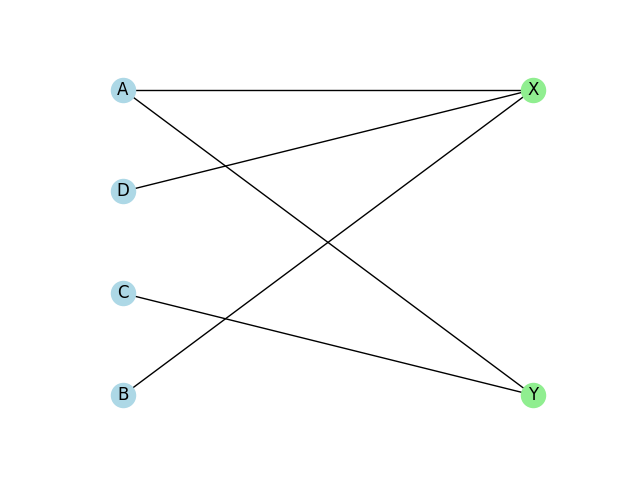
\includegraphics[width=0.6\textwidth]{Graph.png}
\caption{Example of a Bipartite Graph}
\label{fig:bipartite_graph}
\end{figure}

\subsection{Adjacency Matrix}
The adjacency matrix $\mat{A}$ is a square matrix of size $n \times n$, where $n$ is the number of nodes in the graph. For a bipartite graph, the adjacency matrix is partitioned into four blocks, capturing the connections between nodes in $V_1$, nodes in $V_2$, and edges between $V_1$ and $V_2$. The adjacency matrix of a bipartite graph takes the form:

\[
\mat{A} = 
\begin{bmatrix}
\mat{0} & \mat{B} \\
\mat{B}^T & \mat{0}
\end{bmatrix}
\]

where $\mat{0}$ represents the zero matrix and $\mat{B}$ captures the edges connecting $V_1$ and $V_2$. The adjacency matrix provides a concise representation of the graph's structure and facilitates various graph analysis techniques.

\subsection{Eigenvalues of Bipartite Graphs}
The eigenvalues of a bipartite graph's adjacency matrix exhibit an interesting property. Let $\mat{A}$ be the adjacency matrix of a bipartite graph. By definition, a bipartite graph has its vertices divided into two disjoint sets such that all edges connect vertices from different sets. The eigenvalues of $\mat{A}$ appear in pairs of $+a$ and $-a$, where $a$ is a real number. This property holds true due to the specific structure of bipartite graphs and has important implications for understanding their spectral properties.

\begin{figure}[h]
    \centering
    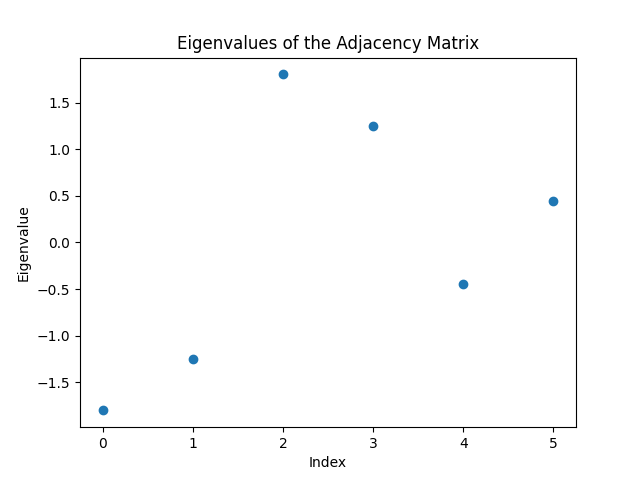
\includegraphics[width=0.6\textwidth]{Eigenvalues.png}
    \caption{Example of a eigenvalues in Complex Plane}
    \label{fig:Eigenvalues}
    \end{figure}
    

\section{Relation with Eigenvalue and Proof}
\begin{theorem}[Eigenvalues of Bipartite Graphs]
Let $\mat{A}$ be the adjacency matrix of a bipartite graph. By definition, a bipartite graph has its vertices divided into two disjoint sets such that all edges connect vertices from different sets. The eigenvalues of $\mat{A}$ appear in pairs of $+a$ and $-a$, where $a$ is a real number.
\end{theorem}

\begin{proof}
We will prove the statement by considering the properties of the adjacency matrix of a bipartite graph.

\begin{enumerate}[label=\textbf{Step \arabic*:}, wide=0pt, leftmargin=!, itemindent=2em]
    \item \textbf{Matrix $A^2$}
    
    Consider the matrix $\mat{A}^2$. The $(i, j)$th entry of $\mat{A}^2$ represents the number of paths of length 2 between vertex $i$ and vertex $j$. In a bipartite graph, there are no direct edges between vertices within the same set, so all entries on the diagonal of $\mat{A}^2$ are zero.
    
    \item \textbf{Equivalence of $A^2v$ and $Av^2$}
    
    For any vector $\vect{v}$, we have $(\mat{A}^2)\vect{v} = \mat{A}(\vect{v}^2)$. This equation can be proven using matrix multiplication.
    
    \item \textbf{Eigenvalue $\lambda$ and eigenvector $\vect{v}$}
    
    Let $\lambda$ be an eigenvalue of $\mat{A}$ with eigenvector $\vect{v}$. By definition, $\mat{A}\vect{v} = \lambda\vect{v}$.
    
    \item \textbf{From $Av = \lambda v$ to $Av^2 = \lambda(Av)$}
    
    Multiply both sides of the equation by $\mat{A}$: $\mat{A}(\mat{A}\vect{v}) = \mat{A}(\lambda\vect{v})$. This yields $\mat{A}^2\vect{v} = \lambda(\mat{A}\vect{v})$.
    
    \item \textbf{Substituting Step 2}
    
    By substituting Step 2, we have $\mat{A}\vect{v}^2 = \lambda(\mat{A}\vect{v})$. This implies that $\lambda$ is an eigenvalue of $\mat{A}^2$ with eigenvector $\vect{v}^2$.
    
    \item \textbf{Non-negativity of $A^2$}
    
    The eigenvalues of $\mat{A}^2$ are non-negative. This is because $\mat{A}^2$ is a non-negative matrix representing the number of paths of length 2 in the bipartite graph.
    
    \item \textbf{Eigenvalue $\lambda$ is non-negative}
    
    Since $\lambda$ is an eigenvalue of $\mat{A}^2$, we have $\lambda \geq 0$.
    
    \item \textbf{Assumption: $\lambda \neq 0$}
    
    Let's assume $\lambda \neq 0$. If $\lambda \neq 0$, then the eigenvector $\vect{v}^2$ is nonzero.
    
    \item \textbf{From $Av = \lambda v$ to $\lambda = \frac{v^TA^Tv}{v^Tv}$}
    
    By the definition of the eigenvalue, we have $\mat{A}\vect{v} = \lambda\vect{v}$. Multiplying both sides of the equation by $\vect{v}^T$, we get $(\vect{v}^T\mat{A}\vect{v}) = \lambda(\vect{v}^T\vect{v})$.
    
    \item \textbf{Symmetric property}
    
    Since $\mat{A}^T = \mat{A}$ for a bipartite graph, we have $\mat{A}^T\vect{v} = \mat{A}\vect{v}$. This implies that $(\vect{v}^T\mat{A}^T\vect{v}) = (\vect{v}^T\mat{A}\vect{v})$.
    
    \item \textbf{Combining Step 9 and Step 10}
    
    Combining steps 9 and 10, we get $\lambda = \frac{v^TA^Tv}{v^Tv}$.
    
    \item \textbf{Eigenvalue $\lambda$ is real}
    
    Since $\lambda = \frac{v^TA^Tv}{v^Tv}$, it follows that $\lambda$ is a real number.
    
    \item \textbf{Conclusion: Eigenvalues appear in pairs}
    
    Therefore, we conclude that the eigenvalues of $\mat{A}$ appear in pairs of $+a$ and $-a$, where $a$ is a real number.
\end{enumerate}

\end{proof}

\begin{figure}[htbp]
  \centering
  \begin{tikzpicture}[scale=1.5]
    % Draw axes
    \draw[->] (-4, 0) -- (4, 0) node[right] {$\text{Re}$};
    \draw[->] (0, -1.5) -- (0, 1.5) node[above] {$\text{Im}$};
    
    % Draw eigenvalues
    \filldraw[color=red] (-2, 0) circle (1pt) node[above] {$-a$};
    \filldraw[color=red] (2, 0) circle (1pt) node[above] {$a$};
    
    % Draw axes labels
    \foreach \x in {-3, -2, ..., 3}
      \draw (\x, 0.1) -- (\x, -0.1) node[below] {$\x$};
    \foreach \y in {-1, 1}
      \draw (0.1, \y) -- (-0.1, \y) node[left] {$\y i$};
  \end{tikzpicture}
  \caption{Eigenvalues of a Bipartite Graph}
  \label{fig:eigenvalues}
\end{figure}
\section{Conclusion for Bipartite Graphs}
In conclusion, the study of bipartite graphs and their eigenvalues holds great promise for understanding graph connectivity, community structure, and various real-world applications. The exploration of eigenvalues provides valuable insights into the robustness, resilience, and behavior of bipartite graphs.

The application of bipartite graphs extends to various domains, including matching and assignment problems, biological networks, and social network analysis. By leveraging the power of eigenvalues, researchers can unravel the hidden intricacies of bipartite graphs and harness their insights to tackle real-world challenges.

Looking to the future, the utilization of bipartite graphs and their eigenvalues is expected to continue advancing. As data becomes increasingly complex and interconnected, bipartite graphs offer a powerful framework for modeling and analyzing large-scale networks. From personalized recommendations to understanding information diffusion, bipartite graphs have the potential to revolutionize various fields and drive innovative solutions.

In conclusion, the study of bipartite graphs and their eigenvalues opens up new avenues for research and practical applications. By delving into the spectral realm of eigenvalues, we can unlock the hidden patterns and structures within bipartite graphs, paving the way for further advancements in graph theory and its applications.

So, let us embrace the power of eigenvalues and embark on a journey to unravel the mysteries of bipartite graphs. With each step, we deepen our understanding of their connectivity, partitioning, symmetry, and dynamics, ultimately enabling us to tackle real-world challenges with confidence and precision.

\section{Clustering in Graphs using Eigenvalues}

    \subsection{What is Clustering?}
    Clustering is the task of grouping objects in a way such that objects belonging to a certain cluster are more similar to each other than to those objects not in the cluster. It is one of the more important techniques in several data analysis fields like pattern recognition, image compression,  bioinformatics, machine learning and several others. Clustering in graphs using eigenvalues and eigenvectors of the adjacency matrix is a widely used technique known as spectral clustering.
    
    \subsection{Spectral Clustering}
    Spectral clustering is a technique with roots in graph theory, where the approach is used to identify communities of nodes in a graph based on the edges connecting them.
    Spectral clustering leverages the spectral properties of the graph Laplacian, which is derived from the adjacency matrix, to partition the graph nodes into cohesive clusters.
    In statistics, spectral clustering techniques make use of the eigenvalues of the similarity matrix of the data to perform dimensionality reduction before clustering in fewer dimensions. The similarity matrix which is provided as the input consists of quantitative assessment of the relative similarity of different pairs of points in the dataset.
    
    \subsection{Basic Terminologies used in Spectral Clustering}
    We will try to explain the basic terminologies in Spectral Clustering using a graph.
        \begin{figure}[ht]
        \centering
            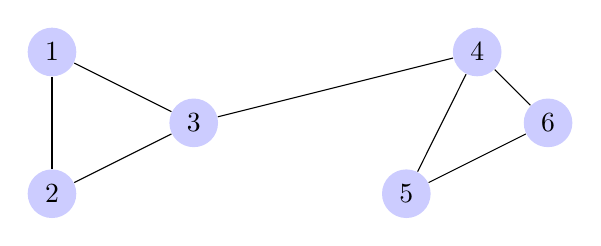
\begin{tikzpicture}[scale=.9,auto=center,every node/.style={circle,fill=blue!20}]
            \node (a1) at (0, 2) {1};
            \node (a2) at (0, 0) {2};
            \node (a3) at (2, 1) {3};
            \node (a4) at (6, 2) {4};
            \node (a5) at (5, 0) {5};
            \node (a6) at (7, 1) {6};
              \draw (a1)--(a2);
              \draw (a1)--(a3);
              \draw (a2)--(a3);
              \draw (a3)--(a4);
              \draw (a4)--(a5);
              \draw (a5)--(a6);
              \draw (a4)--(a6);
            \end{tikzpicture}
            \caption{A simple graph with 6 nodes}
            \label{fig:graph}
        \end{figure}
        \subsubsection{Adjacency and Affinity Matrix $(A)$}
        The graph (or set of data points) can be represented as an Adjacency Matrix, where the row and column indices represent the nodes, and the entries represent the absence or presence of an edge between the nodes (i.e. if the entry in row 0 and column 1 is 1, it would indicate that node 0 is connected to node 1).
        An Affinity Matrix is like an Adjacency Matrix, except the value for a pair of points expresses how similar those points are to each other. If pairs of points are very dissimilar then the affinity should be 0. If the points are identical, then the affinity might be 1. In this way, the affinity acts like the weights for the edges on our graph.\\
        
        \noindent Below is the Adjacency/Affinity matrix of the graph above:
        
        $$ A = 
    	\begin{bmatrix} 
    	0 & 1 & 0 & 0 & 1 & 1 \\
    	1 & 0 & 1 & 0 & 1 & 0 \\
    	0 & 1 & 0 & 1 & 0 & 0 \\
     	1 & 0 & 1 & 0 & 1 & 1 \\
      	0 & 1 & 0 & 1 & 0 & 1 \\
       	0 & 1 & 1 & 0 & 1 & 0 \\
    	\end{bmatrix}
    	\quad
        $$
        \subsubsection{Degree Matrix $(D)$}
        A Degree Matrix is a diagonal matrix, where the degree of a node (i.e. values) of the diagonal is given by the number of edges connected to it. We can also obtain the degree of the nodes by taking the sum of each row in the adjacency matrix.\\
        
        \noindent Below is the Degree matrix of the adjacency matrix we defined above:
        
        $$ D = 
    	\begin{bmatrix} 
    	3 & 0 & 0 & 0 & 0 & 0 \\
    	0 & 2 & 0 & 0 & 0 & 0 \\
    	0 & 0 & 3 & 0 & 0 & 0 \\
     	0 & 0 & 0 & 3 & 0 & 0 \\
      	0 & 0 & 0 & 0 & 2 & 0 \\
       	0 & 0 & 0 & 0 & 0 & 3 \\
    	\end{bmatrix}
    	\quad
        $$
        \subsubsection{Laplacian Matrix $(L)$}
        This is another representation of the graph/data points, which attributes to the beautiful properties leveraged by Spectral Clustering. One such representation is obtained by subtracting the Adjacency Matrix from the Degree Matrix (i.e. $L = D – A$).
        \\
        
        \noindent Below is the Laplacian matrix of the graph we defined above:
        
        $$ L = 
    	\begin{bmatrix} 
    	3 & -1 & 0 & 0 & -1 & -1 \\
    	-1 & 2 & -1 & 0 & -1 & 0 \\
    	-1 & -1 & 3 & -1 & 0 & 0 \\
     	-1 & 0 & -1 & 3 & -1 & -1 \\
      	0 & -1 & 0 & -1 & 2 & -1 \\
       	0 & -1 & -1 & 0 & -1 & 3 \\
    	\end{bmatrix}
    	\quad
        $$
        \begin{enumerate}
            \item \textbf{Spectral Gap}: The first non-zero eigenvalue of $L$ is called the Spectral Gap. The Spectral Gap gives us some notion of the density of the graph.
            \item \textbf{Fiedler Value}: The second eigenvalue of $L$ is called the Fiedler Value, and the corresponding vector is the Fiedler vector. Each value in the Fiedler vector gives us information as to which side of the decision boundary a particular node belongs to.
            \item Using $L$, we find the first large gap between eigenvalues which generally indicates that the number of eigenvalues before this gap is equal to the number of clusters.
        \end{enumerate}
    
    \subsection{Algorithm for spectral clustering in graphs}
    The three major steps involved in spectral clustering are: constructing a similarity graph, projecting data onto a lower-dimensional space, and clustering the data. 
        \begin{enumerate}[label=\textbf{Step \arabic*:}, wide=0pt, leftmargin=!, itemindent=2em]
            \item Form a distance matrix.
            \item Transform the distance matrix into an affinity matrix $A$.
            \item Compute the degree matrix $D$ and the Laplacian matrix $L = D – A$.
            \item Find eigenvalues and eigenvectors of $L$.
            \item With the eigenvectors of $k$ largest eigenvalues computed from the previous step form a matrix.
            \item Normalize the vectors.
            \item Cluster the data points in k-dimensional space.
        \end{enumerate}
    
    \subsection{Why use spectral clustering over other forms of clustering?}
        \begin{enumerate}
            \item \textbf{Flexibility in Handling Complex Data:} Spectral clustering is capable of identifying clusters with complex shapes and structures. It is not limited to spherical or convex clusters like some other algorithms such as k-means. Spectral clustering can handle clusters that are non-linear, disconnected, or overlapping, making it more suitable for a wide range of datasets.
            \item \textbf{Connectivity-Based Clustering:} Spectral clustering takes into account the connectivity or pairwise relationships between data points. Points that are close in proximity but not directly connected can still be assigned to the same cluster. This allows spectral clustering to capture meaningful relationships between data points and identify clusters based on connectivity patterns.
            \item \textbf{Scalability with Sparse Graphs:} Spectral clustering can be particularly efficient when working with sparse graphs. The use of sparse matrix representations and efficient algorithms for eigenvalue computation can help reduce computational costs, making it feasible for large-scale datasets.
        \end{enumerate}.
        \begin{figure}[H]
            \centering
            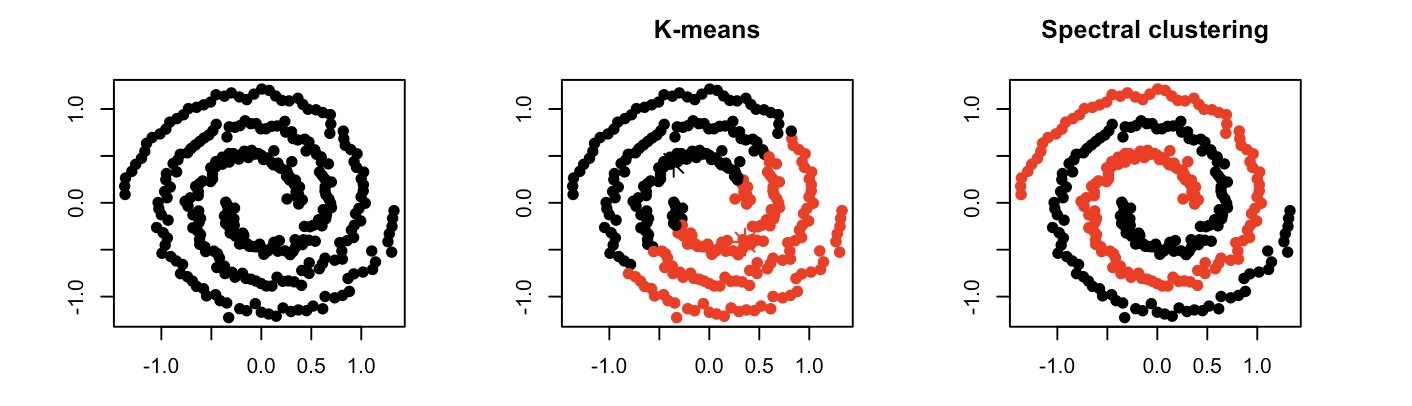
\includegraphics[scale=0.26]{ProsSpectralClust.png}
            \caption{Clustering with different clustering algorithms}
            \label{fig:clustering}
        \end{figure}

    \subsection{Some cons of Spectral Clustering}
        \begin{enumerate}
            \item \textbf{Computational Complexity: }Spectral clustering involves the computation of eigenvalues and eigenvectors of the similarity matrix or Laplacian matrix, which can be computationally expensive for large datasets. The time and memory requirements of spectral clustering can be higher compared to simpler clustering algorithms like k-means.
            \item \textbf{Parameter Selection: }Spectral clustering requires the selection of various parameters, such as the number of clusters (k) and the type of affinity matrix or similarity measure to use. Choosing the optimal values for these parameters can be challenging and may require domain knowledge or trial-and-error experimentation.
            \item \textbf{Lack of Robustness to Noise and Outliers: }Spectral clustering is not inherently robust to noise or outliers in the data. Outliers can influence the computation of the affinity matrix and affect the clustering results. Pre-processing steps or outlier detection techniques may be needed to handle noisy data effectively.
        \end{enumerate}

    \subsection{Uses of Spectral Clustering}
        \begin{enumerate}
            \item \textbf{Recommendation Systems: }Spectral clustering can be employed in recommendation systems to group users or items based on their preferences or similarities. By clustering users or items with similar preferences, personalized recommendations can be made, enhancing the accuracy and relevance of the recommendations.
            \item \textbf{Social network analysis: }Spectral clustering is often used in analyzing social networks to identify communities or groups of nodes with dense connections. By representing the network as a graph and applying spectral clustering, it becomes possible to uncover hidden structures, detect communities, and understand the relationships within the network.
            \item \textbf{Image segmentation: }Spectral clustering can be applied to segment images by grouping pixels or regions with similar characteristics, such as color, texture, or intensity. It has proven to be effective in various computer vision tasks, including object recognition, image compression, and image retrieval.
        \end{enumerate}

\section{Eigenvector Centrality}
    \subsection{What is Eigenvector Centrality in a Graph?}
    In graph theory, eigenvector centrality is a measure of the influence of a node in a network. If a graph node is connected to a node with a high eigenvector centrality score, the graph node in question gets a higher eigenvector centrality score as well. A high eigenvector score means that a node is connected to many nodes who themselves have high scores.

    \subsection{How to compute Eigenvector Centrality?}
    Mathematically, eigenvector centrality is computed using the eigenvector corresponding to the largest eigenvalue of the adjacency matrix of the network. The adjacency matrix represents the connections or relationships between nodes in the network. The eigenvector centrality of a node is given by the corresponding entry in the eigenvector.

    \subsection{Using and Adjacency matrix to compute eigenvector centrality}
    For a graph, $G = (V, E)$, with $V$ vertices let $A = (a_{i, j})$ be the adjacency matrix. Here, $a_{i, j} = 1$ if vertex $i$ is connected to vertex $j$. Otherwise, $a_{i, j} = 0$.\\

    \noindent For this adjacency matrix, the relative centrality score $x_i$ of a vertex $i$ can be expressed as:

    \[x_i = \frac{1}{\lambda} \sum_{j \in V} a_{i, j} \cdot x_j\]

    \noindent The above equation can also be represented as:

    \[Ax = \lambda x\]

    \noindent Here $\lambda$ represents the eigenvalue of the adjacency matrix.\\

    \noindent As, we are measuring the influence of a node in a graph, where the influence cannot be lesser than zero, the eigenvector of the graph (which contains the centrality score of each corresponding node) cannot have entries which are lesser than zero. So, from the Perron Frobenius' theorem, we can say that only the greatest eigenvalue results in the desired centrality scores.
    
    \subsection{Considerations to make while using Eigenvector Centrality}
    \begin{enumerate}
        \item Centrality scores for nodes with no incoming relationships will converge to 0.
        \item Due to missing degree normalization, high-degree nodes have a very strong influence on their neighbors' score.
    \end{enumerate}

    \subsection{Example usage to find Eigenvector Centrality of a graph}
    We can achieve the task of finding the centrality of a graph using Python. A simple Python code fulfils all our need and executes as required to find the centrality score of each node.\\

    \noindent Here is a graph:
    \begin{figure}[ht]
        \centering
            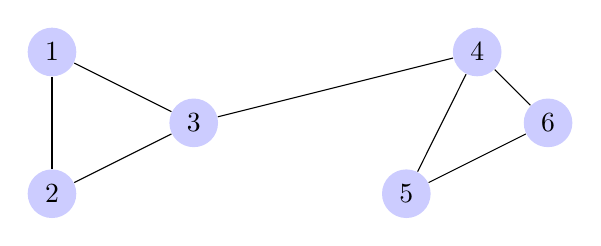
\begin{tikzpicture}[scale=.9,auto=center,every node/.style={circle,fill=blue!20}]
            \node (a1) at (0, 2) {1};
            \node (a2) at (0, 0) {2};
            \node (a3) at (2, 1) {3};
            \node (a4) at (6, 2) {4};
            \node (a5) at (5, 0) {5};
            \node (a6) at (7, 1) {6};
              \draw (a1)--(a2);
              \draw (a1)--(a3);
              \draw (a2)--(a3);
              \draw (a3)--(a4);
              \draw (a4)--(a5);
              \draw (a5)--(a6);
              \draw (a4)--(a6);
            \end{tikzpicture}
            \caption{A graph}
            \label{fig:graph2}
        \end{figure}

    \noindent The centrality score of the graph nodes are as follows: \\
    Node 1: 0.35355343614372065\\
    Node 2: 0.35355343614372065\\
    Node 3: 0.49999993558193184\\
    Node 4: 0.49999993558193184\\
    Node 5: 0.35355343614372065\\
    Node 6: 0.35355343614372065\\

    As we can clearly see, nodes with more edges have higher centrality scores.

    \subsection{Uses of Eigenvector centrality}
    Eigenvector centrality has various applications and has been used in different fields. Here are some notable uses:
    \begin{enumerate}
        \item In a study using data from the Philippines, researchers showed how political candidates' families had disproportionately high eigenvector centrality in local intermarriage networks.
        \item Eigenvector centrality has been extensively applied to study economic outcomes, including cooperation in social networks. In economic public goods problems, a person's eigenvector centrality can be interpreted as how much that person's preferences influence an efficient social outcome.
        \item Eigenvector centrality is commonly employed in social network analysis to identify influential individuals within a social network. Nodes with high eigenvector centrality are considered to have a greater impact and influence on the overall network dynamics. It helps in identifying key individuals who can spread information or influence behavior effectively.
        \item In academic research, eigenvector centrality is used in citation networks to identify influential papers or authors. Nodes with high eigenvector centrality represent papers that are frequently cited by other influential papers, indicating their impact within the research community.
    \end{enumerate}

\end{document}